% !TeX program = xelatex
% Map paths on page 2 are embedded; no external graphics are required.
\documentclass[UTF8,fontset=fandol,12pt,a4paper]{ctexart}
\usepackage[top=20mm,bottom=19mm,left=19mm,right=19mm,headheight=14pt,headsep=9pt,footskip=23pt]{geometry}
\usepackage{fontspec,amsmath,array,tabularx,booktabs,xcolor,colortbl,tikz,fancyhdr,hyperref}
\usetikzlibrary{arrows.meta}
\definecolor{ink}{HTML}{19313C}
\definecolor{muted}{HTML}{465E69}
\definecolor{teal}{HTML}{006963}
\definecolor{lightteal}{HTML}{A6D7C7}
\definecolor{pale}{HTML}{E9F4F0}
\definecolor{amber}{HTML}{AE541E}
\definecolor{sand}{HTML}{E9D7B4}
\definecolor{mist}{HTML}{E6ECEB}
\definecolor{linec}{HTML}{9EAFB1}
\hypersetup{unicode=true,colorlinks=true,urlcolor=teal,linkcolor=teal,pdftitle={Abilene 原八栋园区：电、水、土地与光伏可行性},pdfauthor={IMMC 问题一学生研读资料}}
\setlength{\parindent}{0pt}\setlength{\parskip}{4.5pt}\raggedbottom
\setlength{\tabcolsep}{4pt}\renewcommand{\arraystretch}{1.28}
\newcolumntype{Y}{>{\raggedright\arraybackslash}X}
\newcolumntype{L}[1]{>{\raggedright\arraybackslash}p{#1}}
\newcommand{\ttl}[1]{{\sffamily\bfseries\fontsize{24}{31}\selectfont\color{ink}#1\par}\vspace{1mm}}
\newcommand{\subt}[1]{\par\vspace{2.5mm}{\sffamily\bfseries\fontsize{13}{17}\selectfont\color{teal}#1\par}\vspace{.5mm}}
\newcommand{\captext}[1]{{\small\color{muted}#1\par}}
\newcommand{\tblhead}{\rowcolor{pale}}
\newcommand{\link}[2]{\href{#1}{\textcolor{teal}{#2}}}
\newcommand{\marker}[1]{{\small\sffamily\color{teal}[#1]}}
\newcommand{\metric}[3]{\begin{minipage}[t]{.305\linewidth}{\sffamily\color{muted}\small #1\par}\vspace{1mm}{\sffamily\bfseries\fontsize{25}{28}\selectfont\color{#3}#2}\, {\sffamily\small ha}\end{minipage}}
\pagestyle{fancy}\fancyhf{}\renewcommand{\headrulewidth}{.35pt}\renewcommand{\footrulewidth}{0pt}
\fancyhead[L]{\footnotesize\sffamily\color{muted}IMMC 2027\quad 问题一\enspace/\enspace 场址与容量核查}
\fancyhead[R]{\footnotesize\sffamily\color{muted}ABILENE, TEXAS}
\fancyfoot[L]{\footnotesize\sffamily\color{muted}学生研读资料\quad ·\quad 2026 年 11 月 22 日}
\fancyfoot[R]{\footnotesize\sffamily\color{muted}\thepage\,/\,4}
\begin{document}\color{ink}
\ttl{原八栋园区装得下 429.5 公顷光伏吗？}
在 Abilene，模型为光储分配了 429.5 公顷。若保留原八栋数据中心，只需把各栋的建筑基底加起来，就能判断这套地面方案能否落地。\marker{1–3}\par
\vspace{3mm}
\noindent\colorbox{pale}{\begin{minipage}{\dimexpr\linewidth-2\fboxsep\relax}\vspace{3mm}\hspace{3mm}\metric{园区毛地}{445.15}{ink}\hfill\metric{八栋占地}{36.04}{ink}\hfill\metric{光伏至少缺地}{20.39}{amber}\vspace{3mm}\end{minipage}}
\subt{把两个方案放在同一条面积尺上}
\begin{center}
\begin{tikzpicture}[x=1cm,y=1cm,font=\small\sffamily]
\def\barlen{11.65}
\node[anchor=east] at (-.18,1.02){原八栋布局};\node[anchor=east] at (-.18,.20){模型用地};
\fill[mist] (0,.83) rectangle (\barlen,1.24);\fill[teal] (0,.83) rectangle (.943,1.24);
\fill[lightteal] (0,-.02) rectangle (11.24,.39);\fill[sand] (11.24,-.02) rectangle (\barlen,.39);
\node[anchor=west,fill=mist,inner sep=1pt] at (1.17,1.04){仅扣八栋后，最多剩 409.11 ha};
\node[anchor=west,inner sep=1pt] at (.21,.19){地面光伏 429.50 ha};
\draw[linec] (\barlen,-.14)--(\barlen,-.34);\node[anchor=east] at (\barlen,-.57){毛地 445.15 ha};
\end{tikzpicture}
\end{center}
\captext{深绿为八栋基底，浅褐为光伏方案留给其余一切用途的 15.65 ha。市存图 C1.0 给每栋标出 484,960 ft²。按 $8\times484{,}960\times0.09290304/10{,}000$ 换算，八栋已占 36.04 ha。即使园内除了楼全是空地，也只有 409.11 ha。\textbf{保留八栋楼，429.5 ha 地面光伏放不下。}}
\subt{其余土地用在什么地方}
{\small\begin{tabularx}{\linewidth}{@{}L{27mm}L{29mm}Y@{}}\toprule
\tblhead 用地项目&面积与证据&读数时要留意的范围\\\midrule
八栋建筑基底&36.04 ha｜工程图&只取 1–8 号单层建筑，含楼内机房和辅助空间。9、10 号楼属于后期扩建。\\
两座变电站&新 5.06 ha｜披露\newline 旧约 0.79 ha｜估算&承建商列出 1 GW 新站占 12.5 英亩。旧 200 MW 站取图上外框，缺围界测量。\marker{2,4}\\
道路与停车等&24.05–35.17 ha\newline 图纸间接推算&以图列不透水面积减八栋屋面。1、2 栋共宗且两行相同，两种计法给出两端。纯道路面积仍缺。\\
Longhorn 备用设施&10.27 ha｜整地界\newline 主体约 8.82 ha｜估算&早期工程图列 25.38 英亩施工整地。后者是图示主体，两种面积描述不同阶段的不同边界。\marker{3,5}\\
调蓄池与缓冲带&池区约 9.59 ha\newline 缓冲带约 48.37 ha&池区按图估算，缓冲带来自 2025 年分区测绘图。筛选时整带避让，具体光伏许可待查。\marker{2,6}\\\bottomrule
\end{tabularx}}
\captext{面积有交叠。例如保留整宗运营地时，备用设施大部分已计入宗地。第 2 页改用空间并集扣地。}
\newpage
\ttl{剩下的地能连成多大一块？}
2025 年 7 月的 PDD-181 测绘附件能定位四个规划区块。图载分区面积合计 815.86 英亩，按图形量得约 330.19 ha。它与 Oracle 的 1,100 英亩相差约 115 ha，其余地块的位置、权属和连通关系仍待逐宗核实。\marker{1,6,7}\par
\vspace{1mm}
\begin{minipage}[t]{.485\linewidth}\centering
{\sffamily\bfseries 保留图示运维区}\par
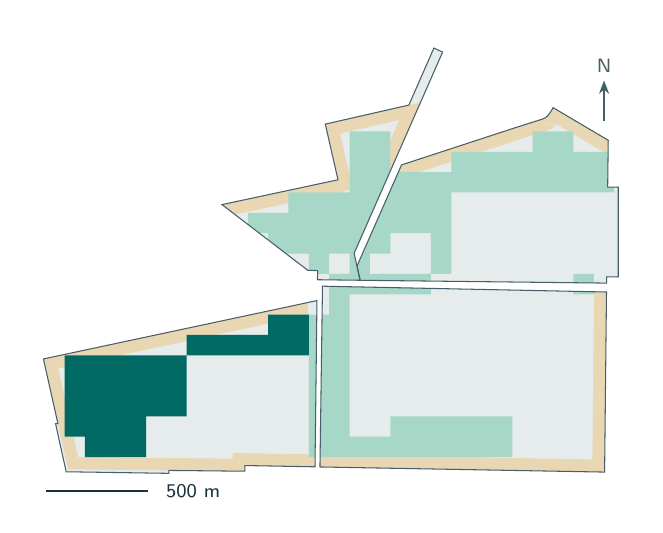
\begin{tikzpicture}[x=1cm,y=1cm,font=\sffamily\scriptsize]
\path[use as bounding box] (0,0) rectangle (7.71,6.06);
\path[even odd rule,fill=mist] (2.757,0.427)--(1.793,0.437)--(1.793,0.400)--(0.489,0.420)--(0.354,1.032)--(0.384,1.031)--(0.200,1.853)--(3.674,2.594)--(3.649,0.483)--(2.759,0.499)--cycle;
\path[even odd rule,fill=mist] (3.712,0.481)--(3.744,2.777)--(7.351,2.703)--(7.327,0.416)--cycle;
\path[even odd rule,fill=mist] (4.748,4.317)--(6.215,4.797)--(6.532,4.897)--(6.573,4.915)--(6.608,4.946)--(6.641,4.989)--(6.673,5.044)--(7.373,4.630)--(7.366,4.034)--(7.500,4.034)--(7.500,2.896)--(7.353,2.896)--(7.353,2.816)--(4.222,2.852)--(4.182,3.032)--cycle;
\path[even odd rule,fill=mist] (3.683,2.975)--(3.558,2.978)--(2.468,3.813)--(3.941,4.128)--(3.780,4.835)--(4.841,5.077)--(5.159,5.801)--(5.270,5.750)--(4.146,3.195)--(4.222,2.852)--(3.680,2.859)--cycle;
\path[even odd rule,fill=sand] (0.483,0.587)--(0.514,0.451)--(2.757,0.427)--(2.759,0.499)--(3.649,0.483)--(3.651,0.640)--(2.604,0.659)--(2.602,0.586)--(0.640,0.607)--(0.389,1.731)--(3.558,2.408)--(3.559,2.569)--(0.200,1.853)--cycle;
\path[even odd rule,fill=sand] (3.715,0.639)--(3.712,0.481)--(7.327,0.416)--(7.351,2.703)--(7.194,2.704)--(7.171,0.576)--cycle;
\path[even odd rule,fill=sand] (4.010,4.887)--(3.780,4.835)--(3.941,4.128)--(2.468,3.813)--(2.633,3.687)--(4.130,4.007)--(3.968,4.716)--(4.719,4.887)--(4.421,4.211)--(4.622,4.277)--(4.989,5.111)--cycle;
\path[even odd rule,fill=sand] (6.068,4.749)--(4.748,4.317)--(4.662,4.123)--(6.264,4.647)--(6.588,4.749)--(6.660,4.781)--(6.719,4.833)--(6.332,4.834)--cycle;
\path[even odd rule,fill=sand] (7.373,4.630)--(7.029,4.833)--(6.719,4.833)--(7.371,4.448)--cycle;
\path[even odd rule,fill=sand] (6.673,5.044)--(6.641,4.989)--(6.608,4.946)--(6.573,4.915)--(6.532,4.897)--(6.332,4.834)--(7.029,4.833)--cycle;
\path[even odd rule,fill=lightteal] (3.721,1.123)--(3.739,2.416)--(3.829,2.416)--(3.829,2.775)--(5.122,2.749)--(5.122,2.674)--(4.088,2.674)--(4.088,0.865)--(4.605,0.865)--(4.605,1.123)--(6.156,1.123)--(6.156,0.606)--(3.714,0.606)--cycle;
\path[even odd rule,fill=lightteal] (3.571,1.382)--(3.571,2.416)--(3.672,2.416)--(3.650,0.606)--(3.571,0.606)--cycle;
\path[even odd rule,fill=lightteal] (3.280,3.191)--(3.054,3.365)--(3.054,3.450)--(2.943,3.450)--(2.795,3.563)--(2.795,3.708)--(3.312,3.708)--(3.312,3.967)--(4.088,3.967)--(4.088,4.742)--(4.605,4.742)--(4.605,4.237)--(4.146,3.195)--(4.222,2.852)--(3.829,2.857)--(3.829,2.933)--(3.682,2.933)--(3.683,2.975)--(3.571,2.978)--(3.571,3.191)--cycle (4.088,2.933)--(4.088,3.191)--(3.829,3.191)--(3.829,2.933)--cycle;
\path[even odd rule,fill=lightteal] (4.252,3.191)--(4.707,4.225)--(5.380,4.225)--(5.380,4.484)--(6.414,4.484)--(6.414,4.742)--(6.931,4.742)--(6.931,4.484)--(7.371,4.484)--(7.366,4.034)--(7.448,4.034)--(7.448,3.967)--(5.380,3.967)--(5.380,2.933)--(5.122,2.933)--(5.122,2.842)--(4.222,2.852)--(4.182,3.032)--cycle (5.122,3.191)--(5.122,3.450)--(4.605,3.450)--(4.605,3.191)--(4.346,3.191)--(4.346,2.933)--(5.122,2.933)--cycle;
\path[even odd rule,fill=lightteal] (7.190,2.706)--(7.190,2.674)--(6.931,2.674)--(6.931,2.711)--cycle;
\path[even odd rule,fill=lightteal] (6.931,2.821)--(6.931,2.933)--(7.190,2.933)--(7.190,2.818)--cycle;
\path[even odd rule,fill=teal] (0.986,0.606)--(0.727,0.606)--(0.727,0.865)--(0.469,0.865)--(0.469,1.899)--(2.020,1.899)--(2.020,1.123)--(1.503,1.123)--(1.503,0.606)--cycle;
\path[even odd rule,fill=teal] (3.054,2.157)--(3.054,2.416)--(3.571,2.416)--(3.571,1.899)--(2.020,1.899)--(2.020,2.157)--cycle;
\path[even odd rule,draw=muted,line width=.38pt] (7.366,4.034)--(7.373,4.630)--(6.673,5.044)--(6.641,4.989)--(6.608,4.946)--(6.573,4.915)--(6.532,4.897)--(6.215,4.797)--(4.748,4.317)--(4.182,3.032)--(4.222,2.852)--(7.353,2.816)--(7.353,2.896)--(7.500,2.896)--(7.500,4.034)--cycle;
\path[even odd rule,draw=muted,line width=.38pt] (7.351,2.703)--(3.744,2.777)--(3.712,0.481)--(7.327,0.416)--cycle;
\path[even odd rule,draw=muted,line width=.38pt] (3.649,0.483)--(3.674,2.594)--(0.200,1.853)--(0.384,1.031)--(0.354,1.032)--(0.489,0.420)--(1.793,0.400)--(1.793,0.437)--(2.757,0.427)--(2.759,0.499)--cycle;
\path[even odd rule,draw=muted,line width=.38pt] (5.270,5.750)--(5.159,5.801)--(4.841,5.077)--(3.780,4.835)--(3.941,4.128)--(2.468,3.813)--(3.558,2.978)--(3.683,2.975)--(3.680,2.859)--(4.222,2.852)--(4.146,3.195)--cycle;
\draw[-{Stealth[length=1.7mm]},line width=.55pt,muted] (7.32,4.88)--(7.32,5.39);
\node[muted] at (7.32,5.58){N};
\draw[ink,line width=.7pt] (.23,.17)--(1.523,.17);
\node[anchor=west,ink] at (1.633,.17){500 m};
\end{tikzpicture}\par
{\small 最大一块\enspace\textbf{39.6 ha}}\end{minipage}\hfill
\begin{minipage}[t]{.485\linewidth}\centering
{\sffamily\bfseries 保留整宗运营地}\par
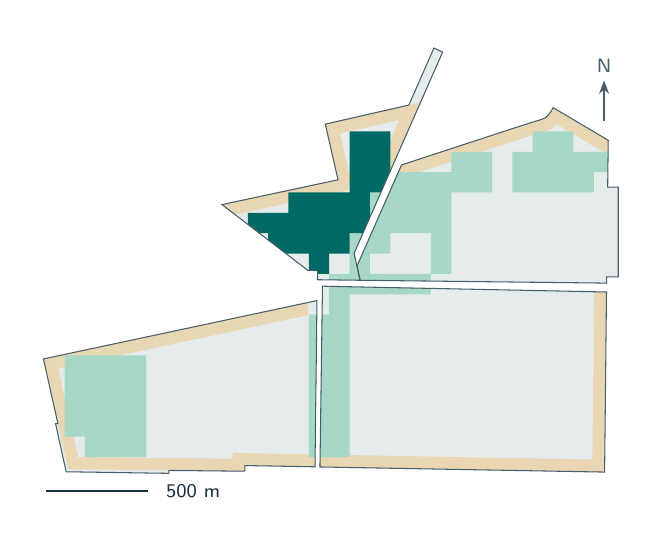
\begin{tikzpicture}[x=1cm,y=1cm,font=\sffamily\scriptsize]
\path[use as bounding box] (0,0) rectangle (7.71,6.06);
\path[even odd rule,fill=mist] (2.757,0.427)--(1.793,0.437)--(1.793,0.400)--(0.489,0.420)--(0.354,1.032)--(0.384,1.031)--(0.200,1.853)--(3.674,2.594)--(3.649,0.483)--(2.759,0.499)--cycle;
\path[even odd rule,fill=mist] (3.712,0.481)--(3.744,2.777)--(7.351,2.703)--(7.327,0.416)--cycle;
\path[even odd rule,fill=mist] (4.748,4.317)--(6.215,4.797)--(6.532,4.897)--(6.573,4.915)--(6.608,4.946)--(6.641,4.989)--(6.673,5.044)--(7.373,4.630)--(7.366,4.034)--(7.500,4.034)--(7.500,2.896)--(7.353,2.896)--(7.353,2.816)--(4.222,2.852)--(4.182,3.032)--cycle;
\path[even odd rule,fill=mist] (3.683,2.975)--(3.558,2.978)--(2.468,3.813)--(3.941,4.128)--(3.780,4.835)--(4.841,5.077)--(5.159,5.801)--(5.270,5.750)--(4.146,3.195)--(4.222,2.852)--(3.680,2.859)--cycle;
\path[even odd rule,fill=sand] (0.483,0.587)--(0.514,0.451)--(2.757,0.427)--(2.759,0.499)--(3.649,0.483)--(3.651,0.640)--(2.604,0.659)--(2.602,0.586)--(0.640,0.607)--(0.389,1.731)--(3.558,2.408)--(3.559,2.569)--(0.200,1.853)--cycle;
\path[even odd rule,fill=sand] (3.715,0.639)--(3.712,0.481)--(7.327,0.416)--(7.351,2.703)--(7.194,2.704)--(7.171,0.576)--cycle;
\path[even odd rule,fill=sand] (4.010,4.887)--(3.780,4.835)--(3.941,4.128)--(2.468,3.813)--(2.633,3.687)--(4.130,4.007)--(3.968,4.716)--(4.719,4.887)--(4.421,4.211)--(4.622,4.277)--(4.989,5.111)--cycle;
\path[even odd rule,fill=sand] (6.068,4.749)--(4.748,4.317)--(4.662,4.123)--(6.264,4.647)--(6.588,4.749)--(6.660,4.781)--(6.719,4.833)--(6.332,4.834)--cycle;
\path[even odd rule,fill=sand] (7.373,4.630)--(7.029,4.833)--(6.719,4.833)--(7.371,4.448)--cycle;
\path[even odd rule,fill=sand] (6.673,5.044)--(6.641,4.989)--(6.608,4.946)--(6.573,4.915)--(6.532,4.897)--(6.332,4.834)--(7.029,4.833)--cycle;
\path[even odd rule,fill=lightteal] (0.727,0.606)--(0.727,0.865)--(0.469,0.865)--(0.469,1.899)--(1.503,1.899)--(1.503,0.606)--cycle;
\path[even odd rule,fill=lightteal] (3.717,0.865)--(3.739,2.416)--(3.829,2.416)--(3.829,2.775)--(5.122,2.749)--(5.122,2.674)--(4.088,2.674)--(4.088,0.606)--(3.714,0.606)--cycle;
\path[even odd rule,fill=lightteal] (3.571,1.123)--(3.571,2.416)--(3.672,2.416)--(3.650,0.606)--(3.571,0.606)--cycle;
\path[even odd rule,fill=lightteal] (4.182,3.032)--(4.594,3.967)--(4.605,3.967)--(4.605,3.992)--(4.707,4.225)--(5.380,4.225)--(5.380,4.484)--(5.897,4.484)--(5.897,3.967)--(5.380,3.967)--(5.380,2.933)--(5.122,2.933)--(5.122,2.842)--(4.222,2.852)--cycle (5.122,3.191)--(5.122,3.450)--(4.605,3.450)--(4.605,3.191)--(4.346,3.191)--(4.346,2.933)--(5.122,2.933)--cycle;
\path[even odd rule,fill=lightteal] (3.829,2.933)--(4.088,2.933)--(4.088,3.450)--(4.258,3.450)--(4.146,3.195)--(4.222,2.852)--(3.829,2.857)--cycle;
\path[even odd rule,fill=lightteal] (4.372,3.708)--(4.346,3.650)--(4.346,3.967)--(4.486,3.967)--cycle;
\path[even odd rule,fill=lightteal] (6.156,4.225)--(6.156,4.484)--(6.414,4.484)--(6.414,4.742)--(6.931,4.742)--(6.931,4.484)--(7.371,4.484)--(7.368,4.225)--(7.190,4.225)--(7.190,3.967)--(6.156,3.967)--cycle;
\path[even odd rule,fill=teal] (3.683,2.975)--(3.571,2.978)--(3.571,3.191)--(3.280,3.191)--(3.054,3.365)--(3.054,3.450)--(2.943,3.450)--(2.795,3.563)--(2.795,3.708)--(3.312,3.708)--(3.312,3.967)--(4.088,3.967)--(4.088,4.742)--(4.605,4.742)--(4.605,4.237)--(4.486,3.967)--(4.346,3.967)--(4.346,3.650)--(4.258,3.450)--(4.088,3.450)--(4.088,3.191)--(3.829,3.191)--(3.829,2.933)--(3.682,2.933)--cycle;
\path[even odd rule,fill=teal] (4.605,3.992)--(4.605,3.967)--(4.594,3.967)--cycle;
\path[even odd rule,draw=muted,line width=.38pt] (7.366,4.034)--(7.373,4.630)--(6.673,5.044)--(6.641,4.989)--(6.608,4.946)--(6.573,4.915)--(6.532,4.897)--(6.215,4.797)--(4.748,4.317)--(4.182,3.032)--(4.222,2.852)--(7.353,2.816)--(7.353,2.896)--(7.500,2.896)--(7.500,4.034)--cycle;
\path[even odd rule,draw=muted,line width=.38pt] (7.351,2.703)--(3.744,2.777)--(3.712,0.481)--(7.327,0.416)--cycle;
\path[even odd rule,draw=muted,line width=.38pt] (3.649,0.483)--(3.674,2.594)--(0.200,1.853)--(0.384,1.031)--(0.354,1.032)--(0.489,0.420)--(1.793,0.400)--(1.793,0.437)--(2.757,0.427)--(2.759,0.499)--cycle;
\path[even odd rule,draw=muted,line width=.38pt] (5.270,5.750)--(5.159,5.801)--(4.841,5.077)--(3.780,4.835)--(3.941,4.128)--(2.468,3.813)--(3.558,2.978)--(3.683,2.975)--(3.680,2.859)--(4.222,2.852)--(4.146,3.195)--cycle;
\draw[-{Stealth[length=1.7mm]},line width=.55pt,muted] (7.32,4.88)--(7.32,5.39);
\node[muted] at (7.32,5.58){N};
\draw[ink,line width=.7pt] (.23,.17)--(1.523,.17);
\node[anchor=west,ink] at (1.633,.17){500 m};
\end{tikzpicture}\par
{\small 最大一块\enspace\textbf{23.4 ha}}\end{minipage}
\par\centering{\small\textcolor{teal}{\rule{3mm}{2.4mm}}\ 最大候选块\quad\textcolor{lightteal}{\rule{3mm}{2.4mm}}\ 其他候选地\quad\textcolor{sand}{\rule{3mm}{2.4mm}}\ 规划缓冲带\quad\textcolor{mist}{\rule{3mm}{2.4mm}}\ 分区底图}\par\raggedright
\captext{两图同尺度，用 100 m 网格显示。候选地覆盖整格至少一半才着色，窄边可能省去。下表按原多边形量算。候选地还需核坡度、检修间距和逐块许可。}
\subt{对已覆盖的部分，每平方米只扣一次}
{\small\begin{tabularx}{\linewidth}{@{}L{35mm}rrY@{}}\toprule
\tblhead 净增扣除面积（ha）&按图示运维区&按整宗运营地&怎样划界\\\midrule
八栋及其运维空间&127.07&179.61&前者取楼群、设备场和内部通道轮廓，后者保留七宗运营地。\\
两座变电站&5.85&5.85&新站形状受披露面积约束，旧站取图示范围。\\
备用设施／调蓄池&8.82／9.59&0.05／0.46&整宗保留时，绝大部分已在上一层内。\\
主要通道／规划缓冲带&7.57／43.68&6.45／44.67&主要通道宽取 12 m，缓冲带扣除与前项重叠后的余额。\\
市洪泛区叠加&0.00&0.00&市 GIS 两档洪泛区与四块相交面积均为零。\marker{8}\\\midrule
\tblhead 剩余土地合计&\textbf{127.62}&\textbf{93.10}&含各个相互分隔的地块。\\
\tblhead 最大连续候选块&\textbf{39.58}&\textbf{23.36}&由原始余地剔除约 10 m 以下的窄连接后量算。\\\bottomrule
\end{tabularx}}
\captext{主要通道按 12 m 推得区内毛占地 7.59 ha。将宽度改为 8 m 或 16 m，左图最大块约为 39.97 或 39.19 ha，右图两次均约 23.36 ha。两列代表不同的运维保留方案，全园最大连续地仍待核定。}
\par 按仓库的 8.9 英亩/MWac 粗算，两块地分别只对应约 \textbf{11.0} 和 \textbf{6.5 MWac} 光伏装机。换成全天可保障的 IT 功率，还需逐时计算。
\newpage
\ttl{把电、水、土地换算成同一个单位}
问题一要求的是给定地点能持续支撑多少 \textbf{MW IT}，即服务器等 IT 设备的功率。设施总功率还要包含制冷和供配电损耗。比较三种资源上限时，要用同一建设阶段、同一供电可靠性和同一水量口径。
\subt{表一\quad 原八栋楼阶段能支撑多大规模？}
{\small\begin{tabularx}{\linewidth}{@{}L{13mm}L{48mm}L{45mm}Y@{}}\toprule
\tblhead 资源&已有资料&代入情景后&仍缺的数据\\\midrule
电&项目公布 1,200 MW 并网规模，原园区燃机最终作备用。\marker{1,9}&若全额持续交付，设施与 IT 的满载倍率 $k=1.41$，可支撑 \textbf{851.1 MW IT}。&同阶段可保障的电力、限电条件和设计满载倍率。\\
水&采用闭式冷却，披露的维护补水为每栋每年约 12,625 美制加仑。\marker{1}&若全站取水强度为 0.50 L/kWh IT，维持 824 MW IT 需 \textbf{412 m³/h}。&枯水或高温期送到场址的流量，以及同期全站取水强度。\\
土地&毛地 445.15 ha，八栋基底 36.04 ha。四个可核界区块的最大候选块见第 2 页。&用修正系数，按同一布局从零规划 824 MW IT，含新站需 \textbf{122.16 ha}。&完整宗地范围、生态限制及同一规模下的设施用地关系。\\\bottomrule
\end{tabularx}}
\captext{仓库所收 Epoch 时间线在 2026-11-01 估计 824 MW IT、1,154 MW 设施功率。按 $k=1.41$ 反算需要 1,161.84 MW。并网数量级相符，水量和净地仍缺，真实三资源联合上限待定。\marker{10}}
\subt{表二\quad 给同一假想地块加一种发电方式}
{\small\begin{tabularx}{\linewidth}{@{}L{25mm}rrrrY@{}}\toprule
\tblhead 方案&新增装机 MW&用地 ha&联合 MW IT&先触顶&优先验证\\\midrule
纯网电参照&0&0&70.92&电&100 MW 是否可持续交付。\\
湿冷煤电&200&40&74.11&水&取水系数和最低稳定出力。\\
干冷燃气&200&20&212.77&电&供气、投运年份及常态运行资格。\\
风电加储能&13.33&400&71.09&电&连续低风期、间距用地能否共享。\\
光伏加储能&119.25&429.5&73.08&电&连续阴天、候选地大小与电池用地。\\\bottomrule
\end{tabularx}}
\captext{四行均含 100 MW 持续网电。案例取水 633.1 m³/h 来自把 2030 年市级规划盈余均摊、全额给园区的假设。风光电池取装机的 25\%、时长 4 h，并要求 1 月 29 日的 24 小时循环运行。煤气均假设机组已投运。\marker{9,10}}
\subt{为什么光伏占了几乎整块地？}
地价和占地代价未进入目标。模型允许把园区毛地重新分给光伏，网电已有 100 MW，光储在选定设计日仅再持续提供 3.04 MW 设施电力，联合容量比纯网电多 \textbf{2.16 MW IT}。同一候选集去掉网电，光伏会用到 439.7 ha，仍只能支撑约 2.21 MW IT。\marker{10}
\newpage
\ttl{固定用地怎样扣，下一步怎样验？}
\subt{先统一变电站的面积边界}
承建商确认新站占 12.5 英亩，开发商原总图与市规划资料均支持把它列为园区配套。税务协议中的开发商保留地含一座容量未注明的变电站，税惠区为 940.89 英亩。与 Oracle 的 1,100 英亩仍缺逐宗对照。先把新站全在界内作为情景，允许界内比例 $f$ 在 0 到 1 之间变化。\marker{1,2,4,6,7}
\[
 A_0=fA_{\rm station},\qquad a=\frac{A_{\rm gross}-fA_{\rm station}}{P_{\rm ref}},\qquad
 P_{\rm land}=\frac{A_{\rm usable}-A_0-A_{\rm generation}}{a}.
\]
仓库的面积公式显式扣一次 $A_0$。若单位用地仍用毛地标定，站地还会随每 MW 分摊。取 $f=1$，用布局假设得到的 $P_{\rm ref}=3{,}096.768$ MW IT，系数从 0.143748 降至 0.1421145 ha/MW IT。824 MW IT 的需地从 123.51 降至 122.16 ha。光储在原候选集重选后用地由 429.5 变为 429.7 ha，容量只多约 1 kW IT。\marker{10}
\subt{学生可以怎样修订第一问}
\textbf{先改用地约束。} 保留原八栋的情景应先锁定已占用土地。若要求一块连续光伏场，另加 $A_{\rm PV}\leq A_{\rm max\ patch}$，若容许分片，可逐块设面积变量并计入各片间距和接入成本。整园上限检验与局部分区结果各有自己的空间范围。\par
\textbf{再补供电和水量的独立验证。} 用场址保障供电量与枯水期可配送水量计算联合上限。对风光储跨季连续运行，并测留出时段的缺供小时与缺供电量。与题面 950 MW、2,263 MW、5 GW 对比前，先统一 IT／设施功率和投运阶段。\par
\subt{可回查的资料}
{\small\renewcommand{\arraystretch}{1.15}\begin{tabularx}{\linewidth}{@{}L{9mm}Y@{}}\toprule
{[1]}&\link{https://arrington.house.gov/uploadedfiles/final_oracle_oai_data_center_fact_sheet_092225b.pdf\#page=1}{Oracle 场址简报，2025-09-23，第 1–2 页}。八栋、1,100 英亩、维护补水及燃机用途。\\
{[2]}&\link{https://www.esig.energy/wp-content/uploads/2025/05/ESIG_LLTF_PresentationLancium.pdf\#page=6}{Lancium 开发商八栋布局，第 6 页}。与随后工程图的 1–8 栋对应。\\
{[3]}&\link{https://abilenetx.gov/DocumentCenter/View/43833/SP-2026-77-PDF?bidId=\#page=1}{Abilene 市存 SP-2026-77，第 1 页 C1.0}。八栋基底、不透水面积及支持设施。\\
{[4]}&\link{https://www.mortenson.com/projects/abilene-data-center-development}{Mortenson 项目记录}。旧站规模、新站规模与 12.5 英亩的占地披露。\\
{[5]}&\link{https://www.abilenetx.gov/DocumentCenter/View/31589/SP-2024-25-Revision-PDF\#page=4}{Abilene 市存 SP-2024-25 修订图，第 4 页}。Longhorn 施工整地范围。\\
{[6]}&\link{https://abilenetx.api.civicclerk.com/v1/Meetings/GetMeetingFileStream(fileId=4620,plainText=false)\#page=106}{市规划会议附件，2025-07-01，第 106–108 页}。Exhibit A、B、D 对应区块、分区图例、测绘界线。\\
{[7]}&\link{https://gis.taylor-cad.org/server/rest/services/Property_Search_Map/MapServer/0}{Taylor 县估价区宗地 GIS}，\link{https://abilenetx.gov/DocumentCenter/View/39456/Lancium-LLC-Abilene-Second-Amended-and-Restated-Tax-Abatement-Agreement-PDF\#page=4}{市税务协议第 4–5、23–25 页}。运营宗地及不同统计边界。\\
{[8]}&\link{https://services6.arcgis.com/iBFmWI3dYPQqS1KF/ArcGIS/rest/services/City_of_Abilene_Flood_Zones/FeatureServer}{Abilene 城市洪泛 GIS}。1\% 与 0.2\% 年超越概率分层。\\
{[9]}&\link{https://www.crusoe.ai/resources/newsroom/crusoe-expands-ai-data-center-campus-in-abilene-to-1-2-gigawatts}{Crusoe 园区并网说明}，\link{https://www.twdb.texas.gov/waterplanning/rwp/plans/2026/G/RegionG_2026_RWP_VolumeI.pdf\#page=607}{得州 Region G 区域水规划，表 5.33-1、5.33-3}。\\
{[10]}&\link{https://github.com/RL-RedLeaf/AIDC-test/tree/e29f173e6fefb8e29455d2b8aea577f6961dfd37/data/geographic_case_abilene_20261122}{仓库案例 e29f173}。输出 03 为各单项候选，11 为网电敏感性，19–23 为更新的电源组合。\\\bottomrule
\end{tabularx}}
\end{document}
